\chapter{Background}
\section{Early Computing}

\subsection{Pressey and Skinner}
\par The earliest learn

% TODO: fix me
\par Learning applications have been used since the early days of computing. In 1958, BF Skinner \cite{skinner1958teaching} explained how computers could be used to facilitate learning. When Dr. Skinner wrote his paper, computers were already used to test students about subjects that were easy to drill. Dr. Skinner believed that computers would completely revolutionize classrooms. Students would be able to learn at their own pace, with the computer determining the optimal schedule for each student based on how they were performing. Skinner argued that the main advantages of computers as teachers were that students are encouraged "to take an active role in the educational process," 


% NO
and notes that the practice of using automation dates back even to the 1920's with Sidney L. Pressey's automated testing machines. One huge advantage that Pressey noted with automated learning is that students learn at their own pace; one of the toughest challenges teachers face, according to Pressey, is that some students will fall behind while others feel bored because they already understand most of the material being taught. While Pressey's automated teaching methods eventually succumbed to the fact that technology at the time wasn't up to the task of automating education. Instead, Skinner was able to use the technology of his time to more effectively bring computers to the field of education.

% TODO: MAke sure it's clear how this ties into the thesis. Bring up the fact that we're trying to change people's behavior.
\subsection{Behavior and Learning}

% TODO: Define behavior, tie it in to learning, tie it into habits.

\par 

Of course, BF Skinner is famous for his creation of the "Skinner Box," \cite{skinner1963operant} a device that gave simple reinforcement to animals or humans in the lab in order to slowly shape their behavior, through a process known as operant conditioning. When a subject performed well according to the test, they would receive a quick reward, while if they strayed from the purpose of the test, they would not receive a reward. Dr. Skinner argued that "much of what we know [about the learning process] has come from studying the behavior of lower organisms, [and] the results hold surprisingly well for human subjects" \cite{skinner1958teaching}.

\subsection{Variable Ratio Reinforcement Scheduling}
 This method is combined with other interesting motivational techniques such as variable rewards scheduling \cite{ferster1957schedules} \cite{hardy_heyes_1999}, where rewards are not actually doled out on a regular basis exactly according to the behavior of the test subject. Instead, rewards are handed out semi-randomly, varying in quantity and quality, while still mostly rewarding the desired behavior that the researcher is trying to condition. This causes the test subject to become conditioned much faster (See \textbf{\hyperref[fig:variable_ratio]{Figure \ref*{fig:variable_ratio}}}).
 
 \begin{figure}[h]
 	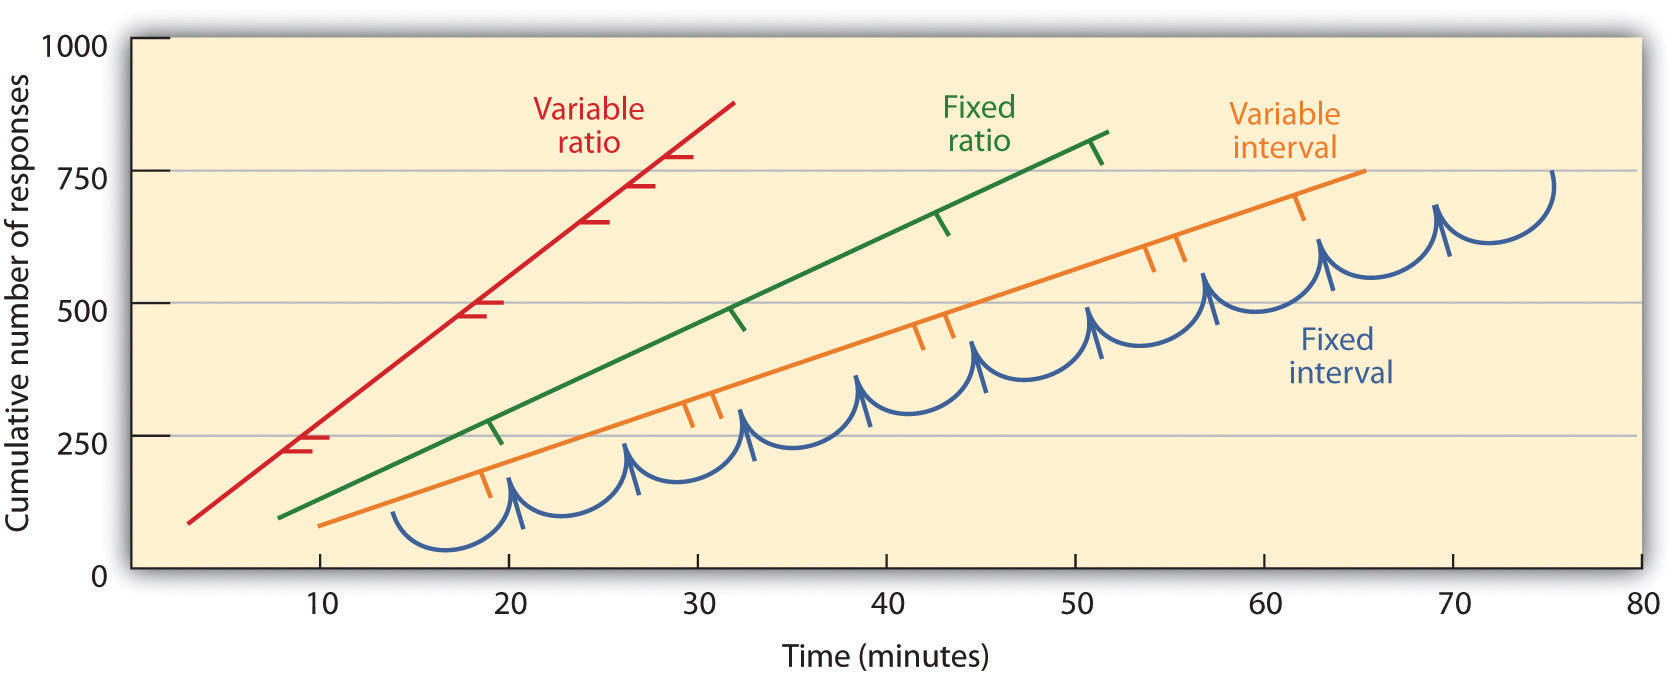
\includegraphics[width=1.0\linewidth]{figures/variable_ratio}
 	\caption{Variable ratio rewards scheduling. Note that as rewards are spaced out randomly, the desired behavior appears much more quickly.}
 	\label{fig:variable_ratio}
 	\cite{hardy_heyes_1999}
 \end{figure}

% TODO: Why is this here? Shouldn't it be in related works
\section{Duolingo}
As mentioned previously in the introduction, Duolingo is an app that already uses several of the processes that we are describing. Duolingo has been shown to be very effective for learning new languages, even perhaps more effective than typical classes. However, the effectiveness of Duolingo is mostly contingent on the motivation of the student. If the student is going to a foreign country soon, Duolingo is the most effective since there is a significant time pressure and pressure to learn the language in order to fit in at whatever country the student is planning to go to \cite{vesselinov2012duolingo}. If, however, the student is simply learning another language for fun, there will be significantly less benefit to them. We must consider this as we develop our educational software; apparently the nature of the student's motivation and their reason for wanting to learn the subject material plays heavily into wheter or not they will be successful in using the app.

\section{Habits}
The study on Duolingo notes how difficult it is to actually get people to use the app. It is extremely hard to change people's habits, taking a lot of time and effort on the user's part to effectively change their behavior. One such strategy around this is to connect one desired "habit" behavior to an existing habit \cite{lally2010habits}. For instance, test subjects in the study by Dr. Lally determined that it was easiest to condition subjects to perform some action by instructing them to perform it right after eating breakfast in the morning. By using the powerful force behind an existing habit, it is possible to "reprogram" your behavior such that a new habit is formed with the new desired behavior.

For instance, if a subject wants to make a habit of cleaning their room, they can make a habit of picking up one piece of clothing after coming home from work for the day. In this way, the habit is driven forward by the regular schedule of coming home at a regular time each day. By associating one behavior with an existing behavior, it is possible to rewire a subject's brain to complete the second behavior far more often.

% TODO Need to read this paper + book in-depth and get a good idea of how habit forming applications go down.
\subsection{New Psychological Theories}
It's interesting to note that the advent of "apps" and habit-forming application has created an essentially new field in psychology \cite{renfree2016don}. In a study, Dr. Renfree argues that the behavior modifications seen in apps like Lift and Memrise actually represent new advances into how habit-forming psychology operates.

% TODO Also expand on this part. The DARK SIDE of gamification, yo
Unfortunately, most of these new effects are actually negative. For instance, Dr. Renfree notes that oftentimes the new habits generated by these apps are "fragile," since they are so dependent on a tight dopamine-based reinforcement loop. As soon as the loop is broken, the brain "loses interest" and the new 
information is deprioritized. This will be an interesting consideration as we develop our application. We want to ensure that the habits and knowledge developed by our app is not simply impermanent, and that it won't be simply "pushed out" by new information.